\documentclass{beamer}
\usetheme{metropolis}           % Use metropolis theme
\title{Deep Checker}

\subtitle{Apprentissage statistique et intelligence artificielle}
\date{}
\author{Arthur Correnson, Igor Martayan, Manon Sourisseau}
\titlegraphic{\hfill
\includegraphics[height=1.5cm]{im/logo.pdf}}
\institute{Projet de Statistiques, ENS, 2021}
\begin{document}

{\metroset{background=dark}\maketitle}

  \begin{frame}{Introduction}
    \begin{columns}
        \column{0.6\textwidth}
        \begin{itemize}
            \item Construction d'une \alert{heuristique} évaluant la qualitée des coups
            \item Nécéssité d'un grand nombre de partie de jeu de dames
        \end{itemize}
        \column{0.4\textwidth}
        \begin{figure}
            \centering
            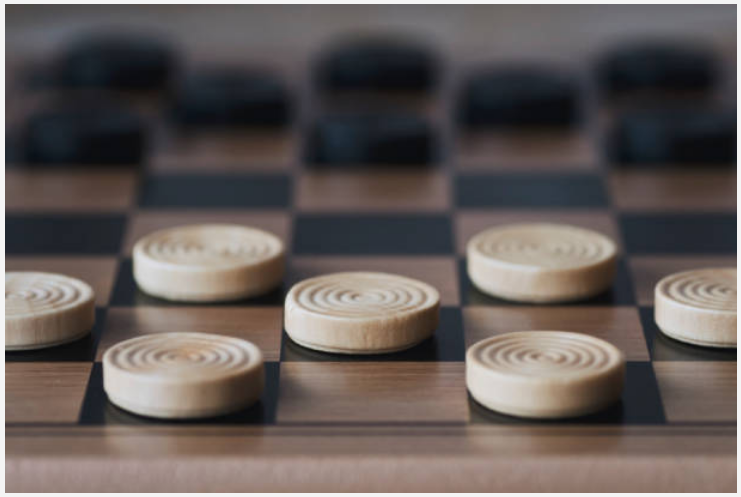
\includegraphics[width=\columnwidth]{im/dames.png}
        \end{figure}
    \end{columns}
  \end{frame}

  \begin{frame}{Plan de la présentation}
    \setbeamertemplate{section in toc}[sections numbered]
    \tableofcontents
\end{frame}

{\metroset{background=dark}\section{Génération de données et simulateur}}
\begin{frame}{Génération de données}
    \begin{itemize}
        \item Besoin d'un \alert{grand nombre de données}
        \item Générer beaucoup de parties \alert{rapidemment} et de manière \alert{compacte} en mémoire
        \item Ecriture d'un simulateur dans le langage \alert{C}
    \end{itemize}
\end{frame}

\begin{frame}{Création d'un simulateur}
    \begin{columns}
        \column{0.6\textwidth}
        \begin{itemize}
            \item 64 cases, 32 cases possibles 
            \item 3 états possibles par cases :\newline
             Vide, pion blanc, pion noir
        \end{itemize}
        Représentation de l'état du plateau par un entier de 64 bits (\alert{2 x 32 bits})
        exemple : 1111 1111 1111 0000 0000 0000 0000 0000 //   0000 0000 0000 0000 0000 1111 1111 1111

        \column{0.4\textwidth}
        \begin{figure}
            \centering
            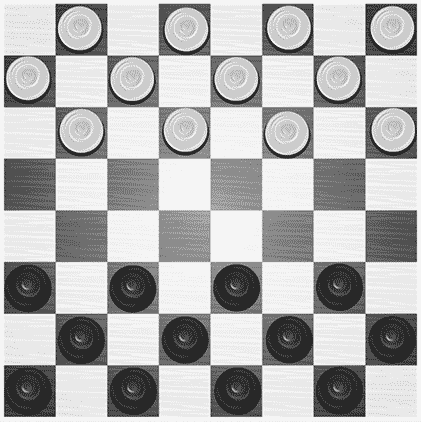
\includegraphics[width=\columnwidth]{im/dames2.png}
        \end{figure}
    \end{columns}
\end{frame}
\begin{frame}{Création d'un simulateur}
    
\end{frame}
{\metroset{background=dark}\section{Modèles et heuristiques}}
\begin{frame}{Modèles et heuristiques}
    
\end{frame}


\end{document}